\titlepageframe % Specific command

% OBJETIVOS %

\begin{tframe}{\textbf{Objetivos}}
	\begin{itemize}
			\item Crear las bases, extensibles y genéricas, de un videojuego \textit{roguelike}
			\item Añadir elementos de accesibilidad, en especial para invidentes, empleando técnicas de Procesamiento de Lenguaje Natural
	\end{itemize}
\end{tframe}

% QUÉ ES UN ROGUELIKE %

\begin{tframe}{\textbf{Objetivos}}
	\begin{itemize}
			\item<+-| alert@+> Crear las bases, extensibles y genéricas, de un videojuego \textit{roguelike}
			\item Añadir elementos de accesibilidad, en especial para invidentes, empleando técnicas de Procesamiento de Lenguaje Natural
	\end{itemize}
\end{tframe}

\begin{tframe}{\textbf{La industria del videojuego}}
	\begin{itemize}
			\item<+-| alert@+> Ha generado 61 billones de dólares en el año 2015, solamente en ventas digitales
	\end{itemize}
\end{tframe}

\begin{tframe}{\textbf{La industria del videojuego}}
	\begin{itemize}
			\item Ha generado 61 billones de dólares en el año 2015, solamente en ventas digitales
			\item<+-| alert@+> Estudios afirman que esta cifra no hará más que crecer hasta el año 2019
	\end{itemize}
\end{tframe}

\begin{tframe}{\textbf{La industria del videojuego}}
	\begin{itemize}
			\item Ha generado 61 billones de dólares en el año 2015, solamente en ventas digitales
			\item Estudios afirman que esta cifra no hará más que crecer hasta el año 2019
			\item<+-| alert@+> Nuevas oportunidades para el crecimiento
	\end{itemize}
\end{tframe}

\begin{tframe}{\textbf{Tiflotecnología}}
	\begin{itemize}
			\item<+-| alert@+> Tecnología de apoyo para invidentes o personas con baja visión.
	\end{itemize}
\end{tframe}

\begin{tframe}{\textbf{Tiflotecnología}}
	\begin{itemize}
			\item Tecnología de apoyo para invidentes o personas con baja visión.
			\item<+-| alert@+> Pocos juegos (en especial \textit{roguelikes}) la tienen en cuenta.
	\end{itemize}
\end{tframe}

\begin{tframe}{\textbf{Videojuegos para invidentes}}
	\begin{itemize}
			\item<+-| alert@+> A Blind Legend
	\end{itemize}
\end{tframe}

\begin{tframe}{\textbf{Videojuegos para invidentes}}
	\begin{itemize}
			\item A Blind Legend
			\item<+-| alert@+> Shades of Doom (adaptación de Doom)
	\end{itemize}
\end{tframe}

\begin{tframe}{\textbf{¿Qué es un \textit{roguelike}?}}
	Género de videojuegos que suele contener las siguientes características:
	\begin{itemize}
		\item<+-| alert@+> Exploración
	\end{itemize}
\end{tframe}

\begin{tframe}{\textbf{¿Qué es un \textit{roguelike}?}}
	Género de videojuegos que suele contener las siguientes características:
	\begin{itemize}
		\item Exploración
		\item<+-| alert@+> Gran dificultad
			\begin{itemize}
				\item Muerte permanente o \textit{permadeath}
				\item Escalable en base al jugador
			\end{itemize}
	\end{itemize}
\end{tframe}

\begin{tframe}{\textbf{¿Qué es un \textit{roguelike}?}}
	Género de videojuegos que suele contener las siguientes características:
	\begin{itemize}
		\item Exploración
		\item Gran dificultad
		\item<+-| alert@+> Aleatoriedad
		\begin{itemize}
			\item Mapas
			\item Enemigos
			\item Objetos
		\end{itemize}
	\end{itemize}
\end{tframe}

\begin{tframe}{\textbf{¿Qué es un \textit{roguelike}?}}
	Género de videojuegos que suele contener las siguientes características:
	\begin{itemize}
		\item Exploración
		\item Gran dificultad
		\item Aleatoriedad
		\item<+-| alert@+> Pseudo-gráficos ASCII
	\end{itemize}
\end{tframe}

\begin{tframe}{\textbf{¿Qué es un \textit{roguelike}?}}
	Frozen depths:
	\begin{figure}[h]
		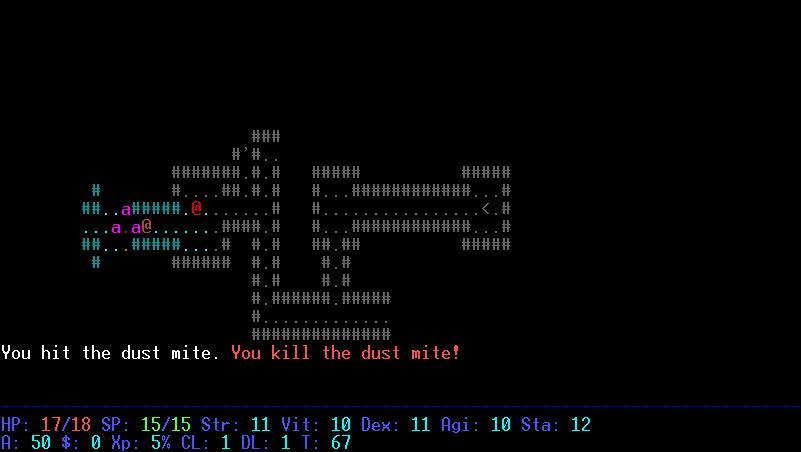
\includegraphics[width=8cm]{../img/frozendepths}
	\end{figure}
\end{tframe}

\begin{tframe}{\textbf{¿Qué es un \textit{roguelike}?}}
	Género de videojuegos que suele contener las siguientes características:
	\begin{itemize}
		\item Exploración
		\item Gran dificultad
		\item Aleatoriedad
		\item Pseudo-gráficos ASCII
		\item<+-| alert@+> Género para aficionados
	\end{itemize}
\end{tframe}

% Roguelike en nuestro proyecto %

\begin{tframe}{\textbf{Elementos \textit{roguelike} en nuestro proyecto}}
	\begin{itemize}
		\item<+-| alert@+> Exploración
			\begin{itemize}
				\item Nuevos objetos
				\item Encontrar el siguiente nivel de la mazmorra
			\end{itemize}
	\end{itemize}
\end{tframe}

\begin{tframe}{\textbf{Elementos \textit{roguelike} en nuestro proyecto}}
	\begin{itemize}
		\item Exploración
		\item<+-| alert@+> Gran dificultad
		\begin{itemize}
			\item Generación de encuentros
			\item Enemigos con distintas IAs
		\end{itemize}
	\end{itemize}
\end{tframe}

\begin{tframe}{\textbf{Elementos \textit{roguelike} en nuestro proyecto}}
	\begin{itemize}
		\item Exploración
		\item Gran dificultad
		\item<+-| alert@+> Aleatoriedad
		\begin{itemize}
			\item Aleatoriedad en mapa y habitaciones
			\item Generador de encuentros: enemigos y objetos
		\end{itemize}
	\end{itemize}
\end{tframe}

% NO ES NADA DIFERENTE %

\begin{tframe}{\textbf{\textit{Roguelikes} comerciales}}
	\begin{itemize}
		\item<+-| alert@+> Género que ha influenciado al sector
	\end{itemize}
\end{tframe}

\begin{tframe}{\textbf{\textit{Roguelikes} comerciales}}
	\begin{itemize}
		\item Género que ha influenciado al sector
		\item<+-| alert@+> Goza de una renovada popularidad, incluso a nivel comercial
	\end{itemize}
\end{tframe}

\begin{tframe}{\textbf{\textit{Roguelikes} comerciales}}
	FTL (Faster Than Light). 2012.
	\begin{figure}[h]
		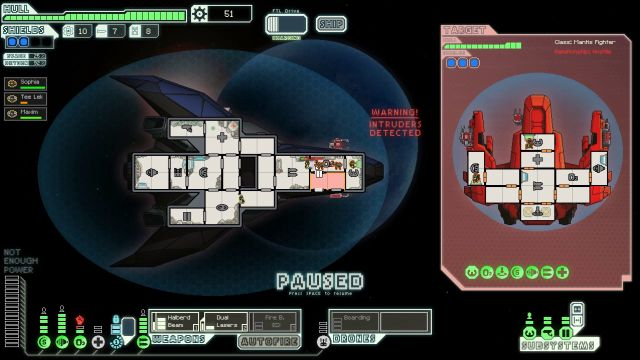
\includegraphics[width=8cm]{../img/ftl}
	\end{figure}
\end{tframe}

\begin{tframe}{\textbf{\textit{Roguelikes} comerciales}}
	Enter the gungeon. 2016.
	\begin{figure}[h]
		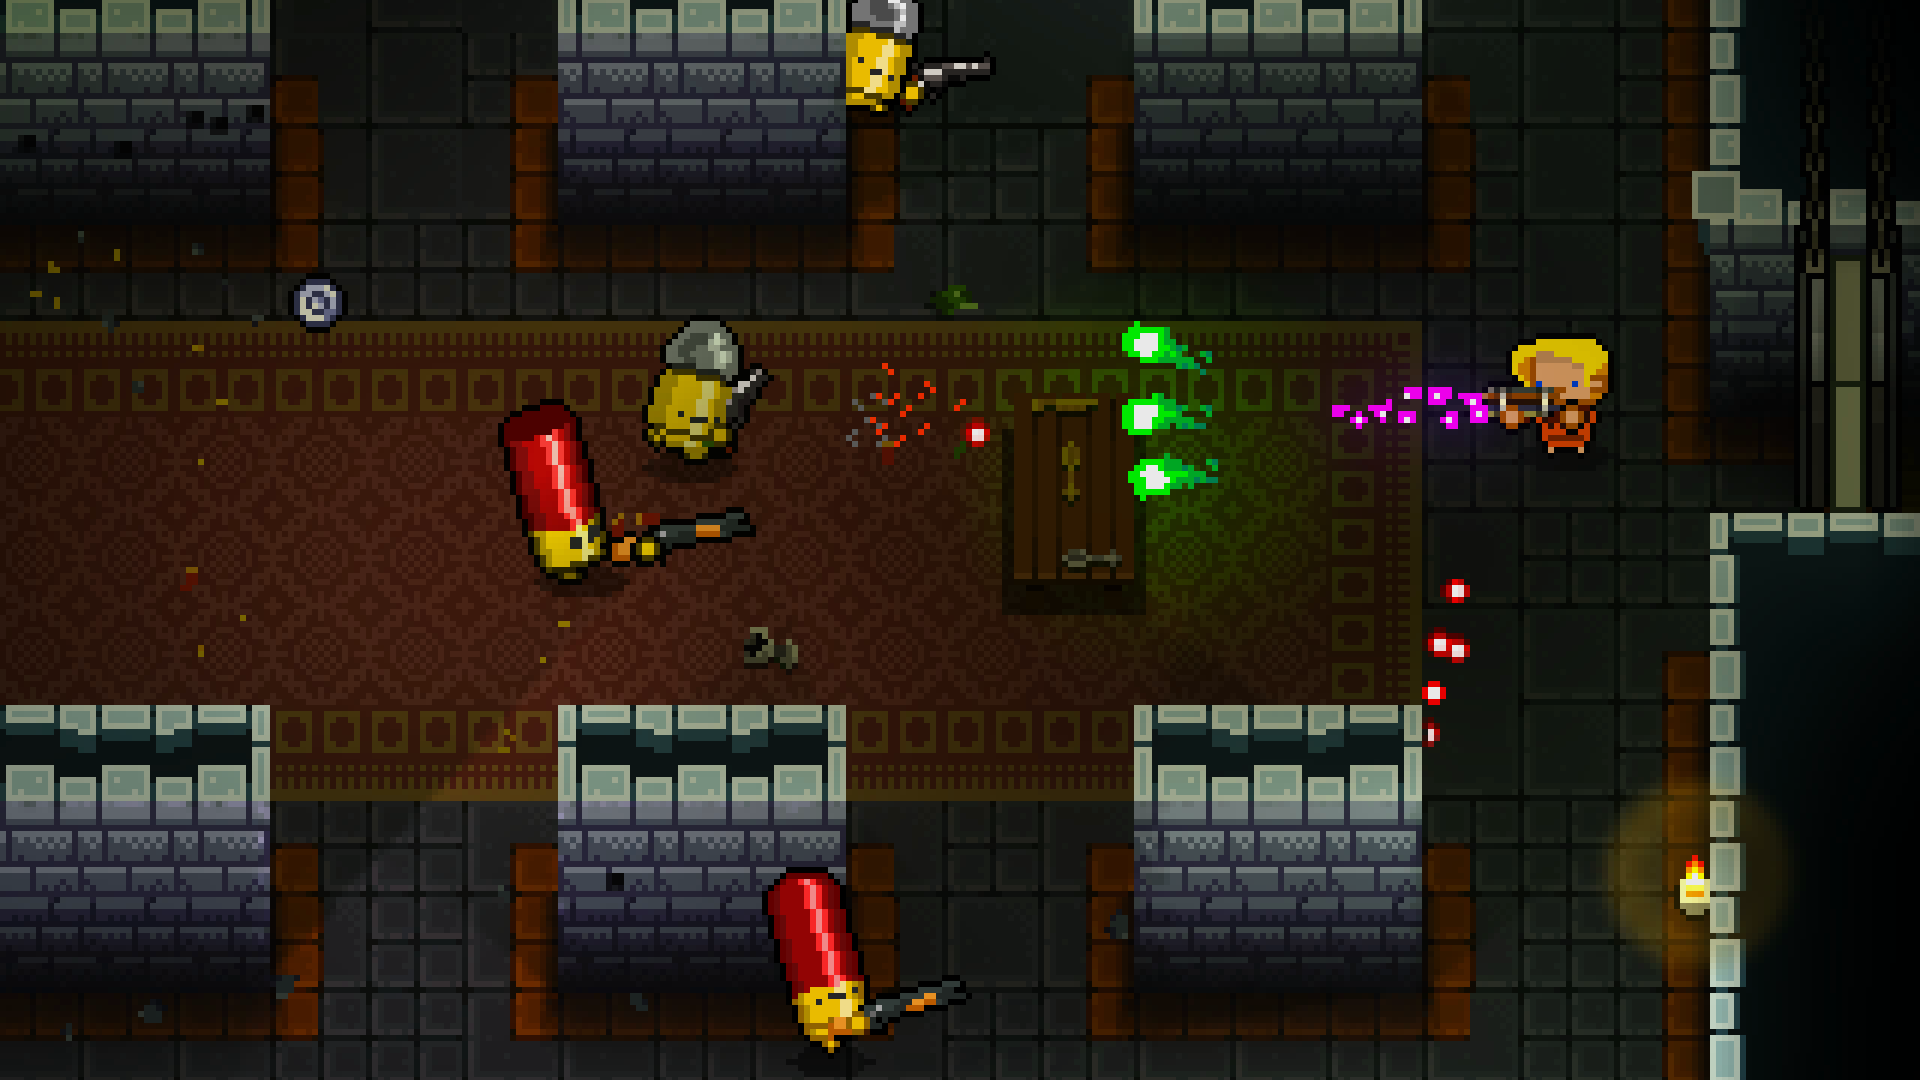
\includegraphics[width=8cm]{../img/enterthegungeon}
	\end{figure}
\end{tframe}

% POR QUÉ DISCRIMINAR? %

\begin{tframe}{\textbf{Objetivos}}
	\begin{itemize}
		\item Crear las bases, extensibles y genéricas, de un videojuego \textit{roguelike}
		\item<+-| alert@+> Añadir elementos de accesibilidad, en especial para invidentes, empleando técnicas de Procesamiento de Lenguaje Natural
	\end{itemize}
\end{tframe}

% ELEMENTOS DE ACCESIBILIDAD EN NUESTRO PROYECTO %

\begin{tframe}{\textbf{Elementos de accesibilidad en nuestro proyecto}}
	\begin{itemize}
		\item<+-| alert@+> Posibilidad de redefinir las teclas
	\end{itemize}
\end{tframe}

\begin{tframe}{\textbf{Elementos de accesibilidad en nuestro proyecto}}
	\begin{itemize}
		\item Posibilidad de redefinir las teclas
		\item<+-| alert@+> Posibilidad de cambiar el tamaño de la fuente (visión reducida)
	\end{itemize}
\end{tframe}

\begin{tframe}{\textbf{Elementos de accesibilidad en nuestro proyecto}}
	\begin{itemize}
		\item Posibilidad de redefinir las teclas
		\item Posibilidad de cambiar el tamaño de la fuente (visión reducida)
		\item<+-| alert@+> Elementos distinguibles por color y forma (daltónicos)
	\end{itemize}
\end{tframe}

\begin{tframe}{\textbf{Elementos de accesibilidad en nuestro proyecto}}
	\begin{itemize}
		\item Posibilidad de redefinir las teclas
		\item Posibilidad de cambiar el tamaño de la fuente (visión reducida)
		\item Elementos distinguibles por color y forma (daltónicos)
		\item<+-| alert@+> Posibilidad de cambiar la paleta de colores (daltónicos)
	\end{itemize}
\end{tframe}

\begin{tframe}{\textbf{Elementos de accesibilidad en nuestro proyecto}}
	Una paleta de colores:
		\begin{figure}[h]
			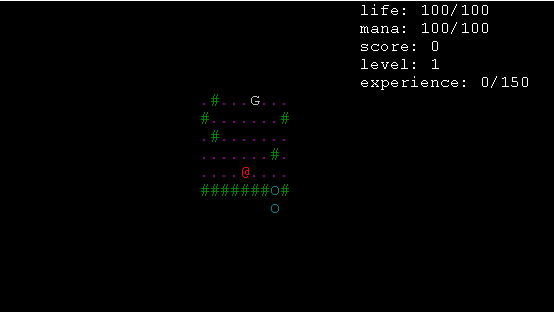
\includegraphics[width=8cm]{../img/paletaColores1.PNG}
		\end{figure}
\end{tframe}

\begin{tframe}{\textbf{Elementos de accesibilidad en nuestro proyecto}}
	Otra paleta de colores:
		\begin{figure}[h]
			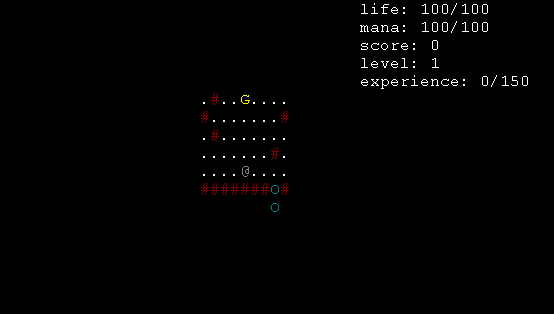
\includegraphics[width=8cm]{../img/paletaColores2.PNG}
		\end{figure}
\end{tframe}

\begin{tframe}{\textbf{Elementos de accesibilidad en nuestro proyecto}}
	\begin{itemize}
		\item Posibilidad de redefinir las teclas
		\item Posibilidad de cambiar el tamaño de la fuente (visión reducida)
		\item Elementos distinguibles por color y forma (daltónicos)
		\item Posibilidad de cambiar la paleta de colores (daltónicos)
		\item<+-| alert@+> Soporte para invidentes
	\end{itemize}
\end{tframe}

% NUESTROS OBJETIVOS PARA DAR SOPORTE A INVIDENTES %

\begin{tframe}{\textbf{Objetivos para dar soporte a invidentes}}
	\begin{itemize}
		\item<+-| alert@+> Generar frases que describan todo lo necesario
	\end{itemize}
\end{tframe}

\begin{tframe}{\textbf{Objetivos para dar soporte a invidentes}}
	\begin{itemize}
		\item Generar frases que describan todo lo necesario
		\item<+-| alert@+> Variedad y expresividad
	\end{itemize}
\end{tframe}

\begin{tframe}{\textbf{Objetivos para dar soporte a invidentes}}
	\begin{itemize}
		\item Generar frases que describan todo lo necesario
		\item Variedad y expresividad
		\item<+-| alert@+> Tener en cuenta la temporalidad
	\end{itemize}
\end{tframe}

\begin{tframe}{\textbf{Objetivos para dar soporte a invidentes}}
	\begin{itemize}
		\item Generar frases que describan todo lo necesario
		\item Variedad y expresividad
		\item Tener en cuenta la temporalidad
		\item<+-| alert@+> Extensibilidad
	\end{itemize}
\end{tframe}

\begin{tframe}{\textbf{Objetivos para dar soporte a invidentes}}
	\begin{itemize}
		\item Generar frases que describan todo lo necesario
		\item Variedad y expresividad
		\item Tener en cuenta la temporalidad
		\item Extensibilidad
		\item<+-| alert@+> No dejar de lado al jugador vidente
	\end{itemize}
\end{tframe}

% ¿CÓMO GENERAR FRASES AUTOMÁTICAMENTE/ALEATORIAMENTE? %

\begin{tframe}{\textbf{¿Cómo generamos las frases?}}
	\begin{itemize}
		\item Gramáticas: Estructura sintáctica
		\item Diccionarios: Léxico
	\end{itemize}
\end{tframe}

\begin{tframe}{\textbf{¿Cómo generamos las frases?}}
	\begin{itemize}
		\item<+-| alert@+> Gramáticas: Estructura sintáctica
		\item Diccionarios: Léxico
	\end{itemize}
\end{tframe}

\begin{frame}[t, fragile]{\textbf{Gramáticas}}
	\vspace*{\fill}
	\begin{Verbatim}
El    héroe   coge   la   espada   metálica
	\end{Verbatim}
	\vspace*{\fill}
\end{frame}

\begin{frame}[t, fragile]{\textbf{Gramáticas}}
	\vspace*{\fill}
	\begin{Verbatim}
El    héroe   coge   la   espada   metálica
	\end{Verbatim}
	\begin{verbatim}
		DET     S       V     D     S        ADJ
	\end{verbatim}
	\vspace*{\fill}
\end{frame}

\begin{frame}[t, fragile]{\textbf{Gramáticas}}
\textbf{En inglés:}

	\begin{Verbatim}
The     hero   picks    the    metallic    sword
	\end{Verbatim}
	\begin{Verbatim}
DET       S      V        D        ADJ       S
	\end{Verbatim}
\vspace*{12px}
\textbf{En español:}
	\begin{Verbatim}
El    héroe   coge   la   espada   metálica
	\end{Verbatim}
	\begin{Verbatim}
DET     S       V     D     S        ADJ
	\end{Verbatim}
\end{frame}

\begin{frame}[t, fragile]{\textbf{Gramáticas}}
Diferentes para cada idioma. Especificadas en archivos JSON:
	\begin{verbatim}
		"S": [
	    	{"DET_1": ""},
	    	{"S_1": ""},
	    	{"V_1": ""},
	    	{"DET_2": ""},
	    	{"S_2": ""},
	    	{"ADJ_1": ""}
		],
	\end{verbatim}
\end{frame}

\begin{frame}[t, fragile]{\textbf{Gramáticas}}
La frase generada puede ser errónea:
	\vspace*{\fill}
		\begin{Verbatim}[commandchars=+\[\]]
La*    héroe   coge   el*   espada   metálico*
		\end{Verbatim}
		\begin{verbatim}
			DET     S       V     D     S        ADJ
		\end{verbatim}
	\vspace*{\fill}
\end{frame}

\begin{frame}[t, fragile]{\textbf{Gramáticas}}
	Debemos añadir restricciones para cada congruencia, diferentes para cada idioma:
	\begin{verbatim}
"S": [
   {"DET_1": ""},
   {"S_1": ""},
   {"ADJ_1": ""}
   ],
"restrictions": [
   {"DET_1.num": "S_1.num"},
   {"DET_1.gen": "S_1.gen"},
   {"ADJ_1.num": "S_1.num"},
   {"ADJ_1.gen": "S_1.gen"}
]
	\end{verbatim}
\end{frame}

% CANTIDAD DE GRAMÁTICAS QUE GENERAMOS %

\begin{frame}[t, fragile]{\textbf{Gramáticas: Importancia de las palabras}}
	Tenemos que generar frases para muchas situaciones diferentes:
	\begin{itemize}
		\item<+-| alert@+> Descripciones en base al jugador
			\begin{itemize}
				\item Inventario
				\item Equipo
				\item Hechizos
				\item Estadísticas (nivel, experiencia, vida...)
			\end{itemize}
	\end{itemize}
\end{frame}

\begin{frame}[t, fragile]{\textbf{Gramáticas: Importancia de las palabras}}
	Tenemos que generar frases para muchas situaciones diferentes:
	\begin{itemize}
		\item Descripciones en base al jugador
		\item<+-| alert@+> Descripciones del mapa
			\begin{itemize}
				\item Enemigos (vida, magia, nivel...)
				\item Posiciones a las que nos podemos mover
				\item Entorno (objetos, puertas, enemigos...)
			\end{itemize}
	\end{itemize}
\end{frame}

\begin{frame}[t, fragile]{\textbf{Gramáticas: Importancia de las palabras}}
	Tenemos que generar frases para muchas situaciones diferentes:
	\begin{itemize}
		\item Descripciones en base al jugador
		\item Descripciones del mapa
		\item<+-| alert@+> Acciones
			\begin{itemize}
				\item Combate cuerpo a cuerpo (tanto del usuario como enemigos)
				\item Ataques mágicos (tanto del usuario como enemigos)
				\item Coger/tirar/equipar/desequipar elementos
			\end{itemize}
	\end{itemize}
\end{frame}

\begin{frame}[t, fragile]{\textbf{Gramáticas: Importancia de las palabras}}
	\vspace*{\fill}
		\begin{Verbatim}[commandchars=+\[\]]
El    +underline[héroe]   coge   la   +underline[espada]   metálica
		\end{Verbatim}
	\vspace*{\fill}
\end{frame}

\begin{frame}[t, fragile]{\textbf{Gramáticas: Importancia de las palabras}}
	Si los núcleos cambian, el resto se adaptan a ellos:
	\vspace*{\fill}
		\begin{Verbatim}[commandchars=+\[\]]
Los    +underline[héroes]   cogen   las   +underline[espadas]   metálicas
		\end{Verbatim}
	\vspace*{\fill}
\end{frame}

% DICCIONARIOS %

\begin{tframe}{\textbf{Diccionarios}}
	\begin{itemize}
		\item Gramáticas: Estructura sintáctica
		\item<+-| alert@+> Diccionarios: Léxico
	\end{itemize}
\end{tframe}

\begin{tframe}{\textbf{Diccionarios}}
	\begin{itemize}
		\item<+-| alert@+> Diccionario para cada idioma
	\end{itemize}
\end{tframe}

\begin{tframe}{\textbf{Diccionarios}}
	\begin{itemize}
		\item Diccionario para cada idioma
		\item<+-| alert@+> Contienen la información necesaria de cada palabra
	\end{itemize}
\end{tframe}

\begin{tframe}{\textbf{Diccionarios}}
	\begin{itemize}
		\item Diccionario para cada idioma
		\item Contienen la información necesaria de cada palabra
		\item<+-| alert@+> Fácilmente traducible y ampliable
	\end{itemize}
\end{tframe}

\begin{frame}[t, fragile]{\textbf{Diccionarios. Ejemplo}}
	\begin{Verbatim}
"goblin": [
    {"num": "sing"},
    {"translation": "goblin"},
    {"numopposite": "goblins"},
    {"gen": "mas"}
],
	\end{Verbatim}
\end{frame}

% GRAMÁTICAS: IDIOMAS DISPONIBLES %

\begin{frame}[t, fragile]{\textbf{Idiomas disponibles}}
	\begin{itemize}
		\item Gallego
		\item Castellano
		\item Inglés
		\item Holandés
	\end{itemize}
\end{frame}

% TEMPORALIDAD %

\begin{tframe}{\textbf{Otros elementos}}
	Otros detalles que tenemos en cuenta:
	\begin{itemize}
		\item Temporalidad
		\item Cambiar el tipo de descripciones (numéricas o no)
		\item Estados que cambian en base a ciertos elementos
	\end{itemize}
\end{tframe}

\begin{tframe}{\textbf{Otros elementos}}
	Otros detalles que tenemos en cuenta:
	\begin{itemize}
		\item<+-| alert@+> Temporalidad
		\item Cambiar el tipo de descripciones (numéricas o no)
		\item Estados que cambian en base a ciertos elementos
	\end{itemize}
\end{tframe}

\begin{tframe}{\textbf{Temporalidad}}
	Tenemos en cuenta la temporalidad:
	\begin{itemize}
		\item<+-| alert@+> Cuando el jugador equipa/desequipa/tira/usa un elemento del inventario
		\begin{figure}[h]
			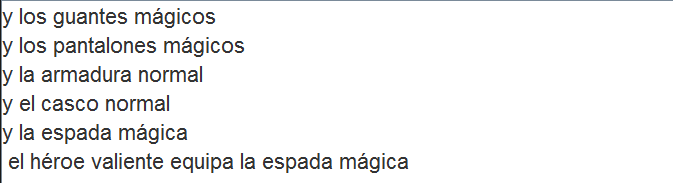
\includegraphics[width=8cm]{../img/temporalidadEquipar.PNG}
		\end{figure}
	\end{itemize}
\end{tframe}

\begin{tframe}{\textbf{Temporalidad}}
	Tenemos en cuenta la temporalidad:
	\begin{itemize}
		\item Cuando el jugador equipa/desequipa/tira/use un elemento del inventario
		\item<+-| alert@+> Durante los combates
		\begin{figure}[h]
			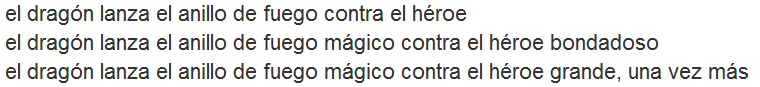
\includegraphics[width=8cm]{../img/temporalidadAtaque.PNG}
		\end{figure}
	\end{itemize}
\end{tframe}

\begin{tframe}{\textbf{Temporalidad}}
	Tenemos en cuenta la temporalidad:
	\begin{itemize}
		\item Cuando el jugador equipa/desequipa/tira/use un elemento del inventario
		\item Durante los combates
		\item<+-| alert@+> Con las descripciones de los enemigos derrotados
		\begin{figure}[h]
			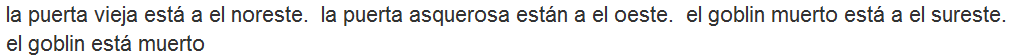
\includegraphics[width=8cm]{../img/enemigosderrotados.PNG}
		\end{figure}
	\end{itemize}
\end{tframe}

% CAMBIAR EL TIPO DE DESCRIPCIONES %

\begin{tframe}{\textbf{Tipos de descripciones}}
	Otros detalles que tenemos en cuenta:
	\begin{itemize}
		\item Temporalidad
		\item<+-| alert@+> Cambiar el tipo de descripciones (numéricas o no)
		\item Estados que cambian en base a ciertos elementos
	\end{itemize}
\end{tframe}

\begin{tframe}{\textbf{Tipos de descripciones}}
	Descripciones sin ser numéricas:
		\begin{figure}[h]
			
\includegraphics[width=8cm]{../img/descripcionnonumerica.PNG}
		\end{figure}
\end{tframe}

\begin{tframe}{\textbf{Tipos de descripciones}}
	Descripciones numéricas explícitas:
		\begin{figure}[h]
			
\includegraphics[width=8cm]{../img/descripcionnumerica.PNG}
		\end{figure}
\end{tframe}

% ESTADOS QUE CAMBIAN EN BASE A OTROS ELEMENTOS %

\begin{tframe}{\textbf{Estados que cambian en base a ciertos elementos}}
	Otros detalles que tenemos en cuenta:
	\begin{itemize}
		\item Temporalidad
		\item Cambiar el tipo de descripciones (numéricas o no)
		\item<+-| alert@+> Estados que cambian en base a ciertos elementos
	\end{itemize}
\end{tframe}

\begin{frame}[c]{\textbf{Estados que cambian en base a ciertos elementos}}
	Las descripciones cambian dependiendo del estado del personaje controlado por el usuario y por los enemigos a los que se enfrenta
	\begin{itemize}
		\item Si el personaje está herido y debilitado (i.e. tiene poca vida), verá a los enemigos como amenazas. Se usarán expresiones como:
		\begin{itemize}
			\item El \textbf{poderoso} enemigo
			\item El \textbf{terrorífico} goblin
		\end{itemize}
		\item Si el personaje está sano (i.e. tiene mucha vida y puede batir a los enemigos fácilmente), los verá como débiles. Se usarán expresiones como:
		\begin{itemize}
			\item El \textbf{endeble} enemigo
			\item El \textbf{insignificante} goblin
		\end{itemize}
	\end{itemize}
\end{frame}

\begin{frame}[c]{}
	\begin{center}
		\Huge Demo
	\end{center}
\end{frame}

% EN CONCLUSIÓN %

\begin{tframe}{\textbf{En conclusión...}}
	Con este sistema de gramáticas y diccionarios podemos:
	\begin{itemize}
		\item<+-| alert@+> Desarrollo de un primer videojuego \textit{roguelike} adaptado a invidentes
	\end{itemize}
\end{tframe}

\begin{tframe}{\textbf{En conclusión...}}
	Con este sistema de gramáticas y diccionarios podemos:
	\begin{itemize}
		\item Desarrollo de un primer videojuego \textit{roguelike} adaptado a invidentes
		\item<+-| alert@+> Implementación de un motor descriptivo multilingüe basado en PLN
	\end{itemize}
\end{tframe}

\begin{tframe}{\textbf{En conclusión...}}
	Con este sistema de gramáticas y diccionarios podemos:
	\begin{itemize}
		\item Desarrollo de un primer videojuego \textit{roguelike} adaptado a invidentes
		\item Implementación de un motor descriptivo multilingüe basado en PLN
		\item<+-| alert@+> Variedad y expresividad en forma
	\end{itemize}
\end{tframe}

\begin{tframe}{\textbf{En conclusión...}}
	Con este sistema de gramáticas y diccionarios podemos:
	\begin{itemize}
		\item Desarrollo de un primer videojuego \textit{roguelike} adaptado a invidentes
		\item Implementación de un motor descriptivo multilingüe basado en PLN
		\item Variedad y expresividad en forma
		\item<+-| alert@+> Fácilmente ampliable
	\end{itemize}
\end{tframe}

\begin{tframe}{\textbf{En conclusión...}}
	Con este sistema de gramáticas y diccionarios podemos:
	\begin{itemize}
		\item Desarrollo de un primer videojuego \textit{roguelike} adaptado a invidentes
		\item Implementación de un motor descriptivo multilingüe basado en PLN
		\item Variedad y expresividad en forma
		\item Fácilmente ampliable
		\item<+-| alert@+> Publicado bajo licencia libre de código abierto: \url{www.github.com/dpenas/roomsgame}
	\end{itemize}
\end{tframe}

\begin{tframe}{\textbf{Y en el futuro...}}
	\begin{itemize}
		\item<+-| alert@+> Desde un punto de vista técnico:
			\begin{itemize}
				\item Ampliar las gramáticas
				\item Integrar recursos lingüísticos de terceros (ej. Wordnet)
				\item Añadir un ``modo resumen'' (\textit{storytelling}, modelización de narrativa)
				\item Contracciones
			\end{itemize}
	\end{itemize}
\end{tframe}

\begin{tframe}{\textbf{Y en el futuro...}}
	\begin{itemize}
		\item Desde un punto de vista técnico:
			\begin{itemize}
				\item Ampliar las gramáticas
				\item Integrar recursos lingüísticos de terceros (ej. Wordnet)
				\item Añadir un ``modo resumen'' (\textit{storytelling}, modelización de narrativa)
				\item Contracciones
			\end{itemize}
		\item<+-| alert@+> Desde un punto de vista de la jugabilidad:
			\begin{itemize}
				\item Mayor variedad de enemigos y otros elementos
				\item Incluir ``modo historia''
				\item Añadir más elementos sonoros
			\end{itemize}
	\end{itemize}
\end{tframe}

\begin{tframe}{\textbf{Agradecimientos}}
	\begin{itemize}
		\item Juan Carlos Buño Suárez (instructor de tiflotecnología de la ONCE)
		\item Usuarios de Reddit \textit{ais523} y \textit{fastfinge}
	\end{itemize}
\end{tframe}

% PREGUNTAS Y GRACIAS %

\begin{frame}[c]{}
	\begin{center}
		\Huge ¡Gracias por su atención!
	\end{center}
\end{frame}

\begin{frame}[c]{}
	\begin{center}
		\Huge ¿Preguntas?
	\end{center}
\end{frame}